\section{Duplication V.S. Scale}
Dealing with large scale VM cloud, one of the most important questions is
whether data duplication will grow with the system scale. 
One hypothesis we have is that when the total number of block increases,
the chance that it being duplicated with another is going to be higher. Thus
we shall get better data reduction with larger scale of data.
Past study\cite{keren08} has suggested that virtual disks with 
operating systems installed should share large amount of software related data,
which indirectly supports this argument.
However, some other data study\cite{middleware11} showed the opposite.

In this experiment we test the complete deduplication under the scenario
that no snapshot backup is involved. To simulate the scale factor,
we start with partial data sets and scale them up by adding disk images.
Complete deduplication is performed at each stage to examine the reduction ratio.
Our DDS data set already contains no snapshot backup data. For VOSS, we simply pick
the earliest snapshot for each VM.

\begin{figure}
  \centering
  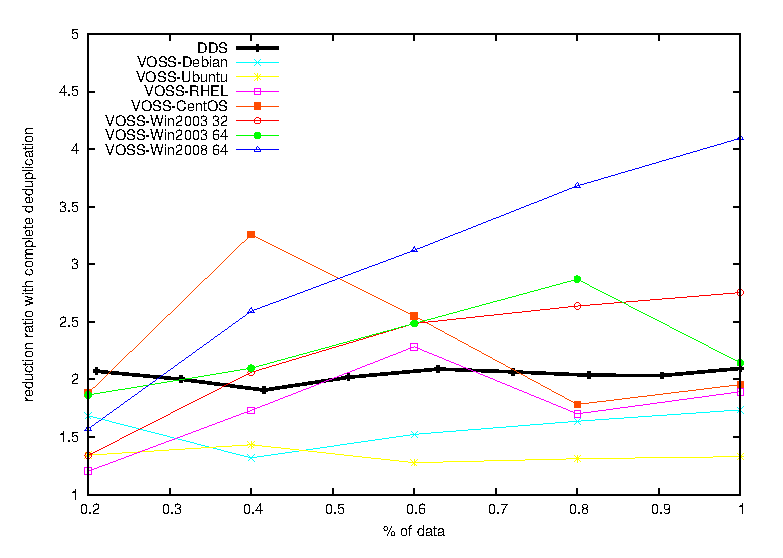
\epsfig{file=dedup_ratio.eps, width=3.2in}
  \caption{Reduction ratio of complete deduplication at different scale}
  \label{fig:scale}
\end{figure}

\emph{Observation 7: Reduction ratio by complete deduplication does not appear to increase with storage scale.}
In general we see almost no increment of reduction ratio along with the data scale, especially
for user generated data, shown as DDS in Figure\ref{fig:scale}, its reduction ratio is always
near 2:1. For OS disks, some Windows distributions appear to have incremental reduction, which is suspected to
because the size of Windows system is much bigger than Linux, thus it has much more redundant
data that widely exist in all VMs. We expect to perform larger scale study on OS disks in future
to obtain better conclusion on this topic.